\documentclass{article}
\usepackage[export]{adjustbox}
\usepackage{graphicx}
\usepackage{fancyvrb}


\title{Reporte Actividad 4}
\author{Andr\'es Rodr\'iguez}
\date{}


\begin{document}

\maketitle

\graphicspath{ {Graphs/} }


\section{Introducci\'on}

En esta pr\'actica se utiliza la herramienta Maxima para construir gr\'aficas de aproximaciones de Taylor de varias funciones. Se muestra la funci\'on aproximada, la gr\'afica de las aproximaciones y el c\'odigo utilizado en Maxima.

\section{Aproximaciones de Taylor}
Se define el polinomio de Taylor de grado n para la funcion $f$ en el punto a, denotado por $P_{n,a}$, como:

$$P_{n,a} = f(a) + \frac{f'(a)}{1!}(x-a) + \frac{f''(a)}{2!}(x-a)^2 + ... + \frac{f^{(n)}(a)}{n!}(x-a)^n. $$
El cual cumple que

$$\lim_{x\to a} \frac{f(x)-P_{n,a}(x)}{(x-a)^n}=0$$
lo que indica que la diferencia entre $f(x)$ y $P_{n,a}(x)$ se hace peque\~na en comparaci\'on con $(x-a)^n$ cuando $x$ tiende a $a$. Lo cual expresa que se puede utilizar el polinomio de Taylor como una muy buena aproximaci\'on a la funci\'on cerca del punto $a$. Al aumentar el orden del polinomio se produce una mejor aproximaci\'on.
\section{Funciones}



\subsection{$f(x)= sin(x)$}
Aproximaci\'on de Taylor de la funci\'on sin(x), alrededor del punto  x=0, de aproximaci\'on 1, 3, 5 y 7.

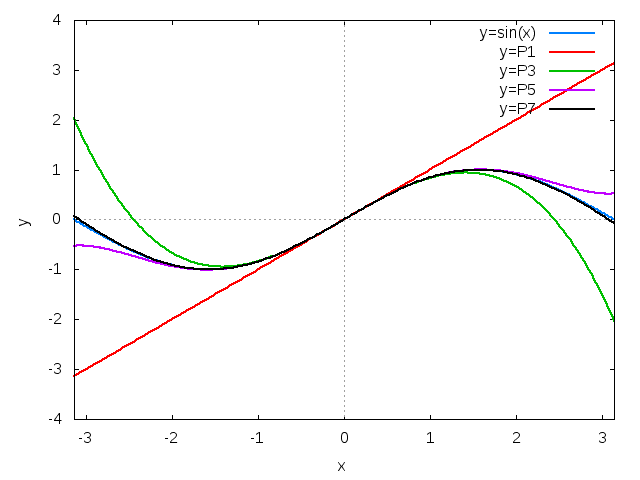
\includegraphics[scale=.5]{sin}

\begin{Verbatim}[frame=single]
/* [wxMaxima batch file version 1] [ DO NOT EDIT BY HAND! ]*/
/* [ Created with http://maxima-online.org ] */

/* [wxMaxima: comment start ]
This solution online http://maxima-online.org/?inc=r-449223125
   [wxMaxima: comment end   ] */

/* [wxMaxima: input   start ] */
f(x):= sin(x);
P1(x):=taylor(f(x), x, 0, 1);
P3(x):=taylor(f(x), x, 0, 3);
P5(x):=taylor(f(x), x, 0, 5);
P7(x):=taylor(f(x), x, 0, 7);
fortran(P1(x));
fortran(P3(x));
fortran(P5(x));
fortran(P7(x));
tex(P1(x));
tex(P3(x));
tex(P5(x));
tex(P7(x));
plot2d ([f(x),P1(x),P3(x),P5(x),P7(x)], 
[x, -%pi, %pi],[style, [lines,2]],
[legend, "y=sin(x)", "y=P1", "y=P3", "y=P5", "y=P7"]);
/* [wxMaxima: input   end   ] */
\end{Verbatim}


\noindent\rule{\textwidth}{1pt}



\subsection{$f(x)= log(1+x)$}
Aproximaci\'on de Taylor de la funci\'on log(1+x), alrededor del punto  x=0, de aproximaci\'on 4, 7, 11, 16.

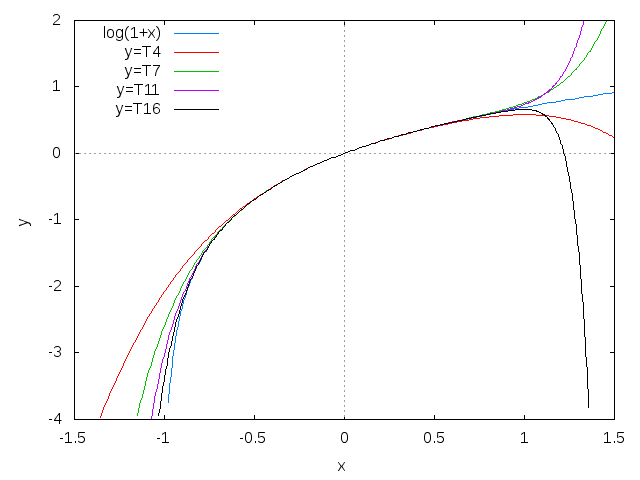
\includegraphics[scale=.5]{log}

\begin{Verbatim}[frame=single]
/* [wxMaxima batch file version 1] [ DO NOT EDIT BY HAND! ]*/
/* [ Created with http://maxima-online.org ] */

/* [wxMaxima: comment start ]
This solution online http://maxima-online.org/?inc=r-1002504485
   [wxMaxima: comment end   ] */

/* [wxMaxima: input   start ] */
f(x):= log(x+1);
T4(x):=taylor(f(x), x, 0, 4);
T7(x):=taylor(f(x), x, 0, 7);
T11(x):=taylor(f(x), x, 0, 11);
T16(x):=taylor(f(x), x, 0, 16);
fortran(T4(x));
fortran(T7(x));
fortran(T11(x));
fortran(T16(x));
tex(T4(x));
tex(T7(x));
tex(T11(x));
tex(T16(x));
plot2d ([f(x),T4(x),T7(x),T11(x),T16(x)],
[x, -1.5, 1.5],[y, -4, 2],[legend, "log(1+x)",
 "y=T4", "y=T7", "y=T11", "y=T16"],
 [gnuplot_preamble,"set key left"]);
/* [wxMaxima: input   end   ] */
\end{Verbatim}


\noindent\rule{\textwidth}{1pt}



\subsection{$f(x)= log(cos(x))$}

Aproximaci\'on de Taylor de la funci\'on log(cos(x)), alrededor del punto  x=0, de aproximaci\'on 4, 7, 11, 16.


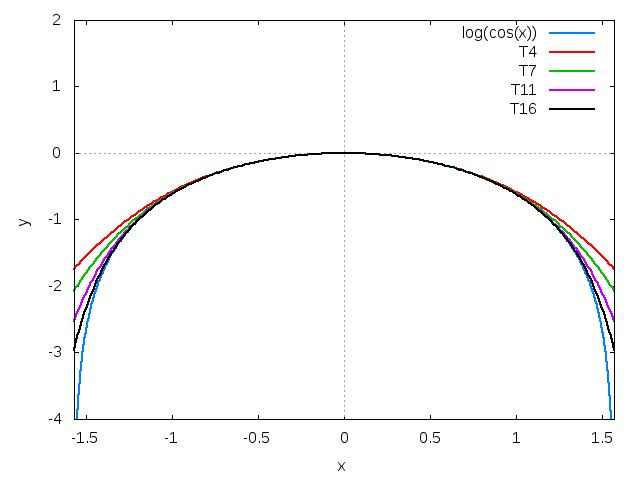
\includegraphics[scale=.5]{logcos}

\begin{Verbatim}[frame=single]
/* [wxMaxima batch file version 1] [ DO NOT EDIT BY HAND! ]*/
/* [ Created with http://maxima-online.org ] */

/* [wxMaxima: comment start ]
This solution online http://maxima-online.org/?inc=r-1285007665
   [wxMaxima: comment end   ] */

/* [wxMaxima: input   start ] */
f(x):= log(cos(x));
T4(x):=taylor(f(x), x, 0, 4);
T7(x):=taylor(f(x), x, 0, 7);
T11(x):=taylor(f(x), x, 0, 11);
T16(x):=taylor(f(x), x, 0, 16);
fortran(T4(x));
fortran(T7(x));
fortran(T11(x));
fortran(T16(x));
tex(T4(x));
tex(T7(x));
tex(T11(x));
tex(T16(x));

plot2d ([f(x),T4(x),T7(x),T11(x),T16(x)],
[x, -%pi/2, %pi/2],[y, -4, 2],
[legend, "log(cos(x))", "T4", "T7", "T11", "T16"],
[style,[lines,2]]);
/* [wxMaxima: input   end   ] */
\end{Verbatim}

\noindent\rule{\textwidth}{1pt}


\subsection{$f(x)= (1+x)e^x$}

Aproximaci\'on de Taylor de la funci\'on $(1+x)e^x$, alrededor del punto  x=0, de aproximaci\'on 4, 7, 11, 16.

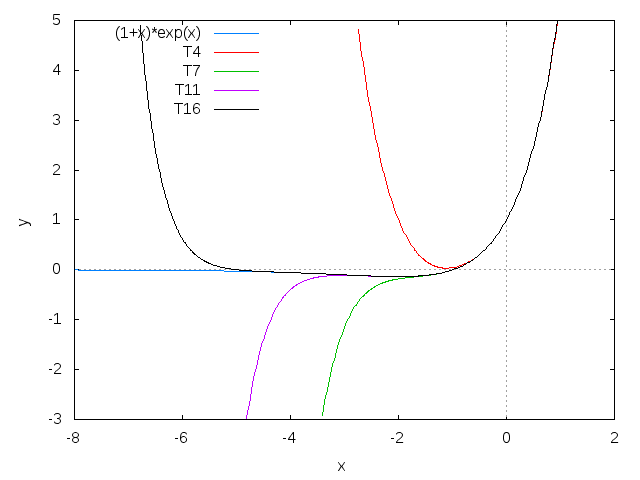
\includegraphics[scale=.5]{xexp}

\begin{Verbatim}[frame=single]
/* [wxMaxima batch file version 1] [ DO NOT EDIT BY HAND! ]*/
/* [ Created with http://maxima-online.org ] */

/* [wxMaxima: comment start ]
This solution online http://maxima-online.org/?inc=r-717215049
   [wxMaxima: comment end   ] */

/* [wxMaxima: input   start ] */
f(x):= (1+x)*exp(x);
T4(x):=taylor(f(x), x, 0, 4);
T7(x):=taylor(f(x), x, 0, 7);
T11(x):=taylor(f(x), x, 0, 11);
T16(x):=taylor(f(x), x, 0, 16);
fortran(T4(x));
fortran(T7(x));
fortran(T11(x));
fortran(T16(x));
tex(T4(x));
tex(T7(x));
tex(T11(x));
tex(T16(x));
plot2d ([f(x),T4(x),T7(x),T11(x),T16(x)],[x, -8, 2],
[y, -3, 5],   [gnuplot_preamble, "set key left"],
[legend, "(1+x)*exp(x)", "T4", "T7", "T11", "T16"]);
/* [wxMaxima: input   end   ] */
\end{Verbatim}



\noindent\rule{\textwidth}{1pt}


\subsection{$f(x)= \frac{e^x}{cos(x)}$}

Aproximaci\'on de Taylor de la funci\'on $\frac{e^x}{cos(x)}$, alrededor del punto  x=0, de aproximaci\'on 4, 7, 11, 16.

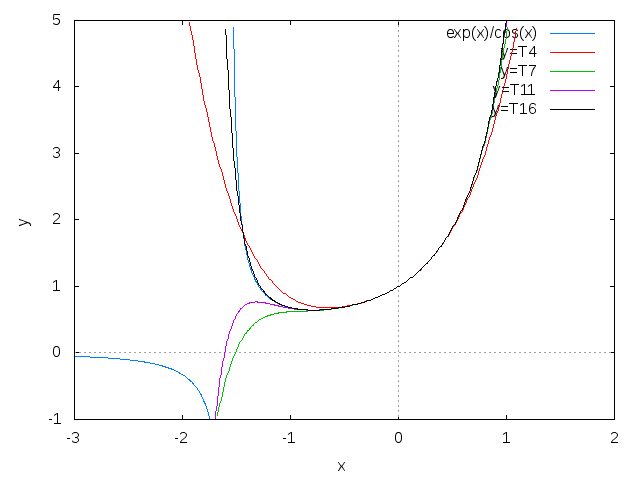
\includegraphics[scale=.5]{exp_cos}

\begin{Verbatim}[frame=single]
/* [wxMaxima batch file version 1] [ DO NOT EDIT BY HAND! ]*/
/* [ Created with http://maxima-online.org ] */

/* [wxMaxima: comment start ]
This solution online http://maxima-online.org/?inc=r-803283332
   [wxMaxima: comment end   ] */

/* [wxMaxima: input   start ] */
f(x):= exp(x)/cos(x);
T4(x):=taylor(f(x), x, 0, 4);
T7(x):=taylor(f(x), x, 0, 7);
T11(x):=taylor(f(x), x, 0, 11);
T16(x):=taylor(f(x), x, 0, 16);
fortran(T4(x));
fortran(T7(x));
fortran(T11(x));
fortran(T16(x));
tex(T4(x));
tex(T7(x));
tex(T11(x));
tex(T16(x));
plot2d ([f(x),T4(x),T7(x),T11(x),T16(x)],[x, -3, 2],
[y, -1, 5],[legend, "exp(x)/cos(x)", 
"y=T4", "y=T7", "y=T11", "y=T16"]);
/* [wxMaxima: input   end   ] */
\end{Verbatim}



\end{document}